\documentclass[12pt,a4paper]{article}
\usepackage[slovene]{babel}
\usepackage{graphicx}
\usepackage{hyperref}
\begin{document}\documentclass[12pt,a4paper]{article}
\usepackage[slovene]{babel}
\usepackage{graphicx}
\usepackage{hyperref}
\begin{document}

\title{Marprom - Pregled obstoječih rešitev}
\author{Leon Bracko, Tijan Eisenhut List}
\date{November 2026}
\maketitle

\section{Uvod}

Naš projekt je povezan z mestnim avtobusnim
prometom Marprom v Mariboru.

Namen projekta je uporabnikom omogočiti
enostaven pregled voznih redov, avtobusnih
linij in drugih informacij o prevozu.

Pregledali smo tri obstoječe digitalne
storitve podjetja Marprom.

\section{Interaktivni vozni redi}

Interaktivni vozni redi omogočajo pregled
avtobusnih linij in odhodov v Mariboru
\cite{vozniredi}.

\textbf{Funkcionalnosti:}
Pregled linij, postajališč in voznih redov.

\textbf{Prednosti:}
Enostaven dostop do informacij o odhodih.

\textbf{Slabosti:}
Za uporabo je potrebna internetna povezava.

\begin{figure}[h]
\centering
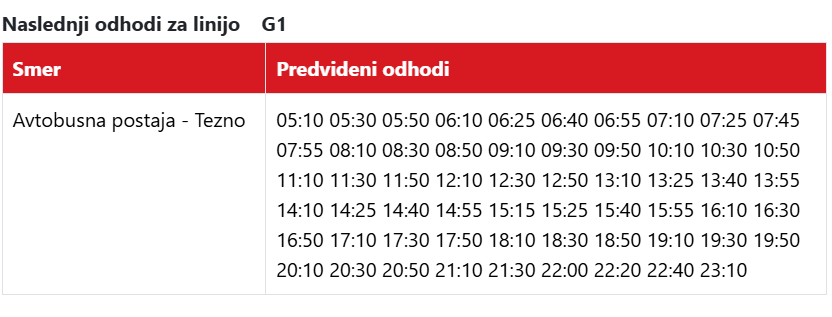
\includegraphics[width=0.8\textwidth]{vozniredi.png}
\caption{Interaktivni vozni redi Marprom}
\end{figure}

\section{M mobilnost}

M mobilnost je mobilna aplikacija za
spremljanje avtobusnega prometa v
Mariboru \cite{mobilnost}.

\textbf{Funkcionalnosti:}
Prikaz avtobusov v realnem času,
pregled odhodov in načrtovanje poti.

\textbf{Prednosti:}
Uporabnik lahko spremlja položaj
avtobusa na zemljevidu.

\textbf{Slabosti:}
Za uporabo potrebujemo pametni telefon
in internetno povezavo.

\begin{figure}[h]
\centering
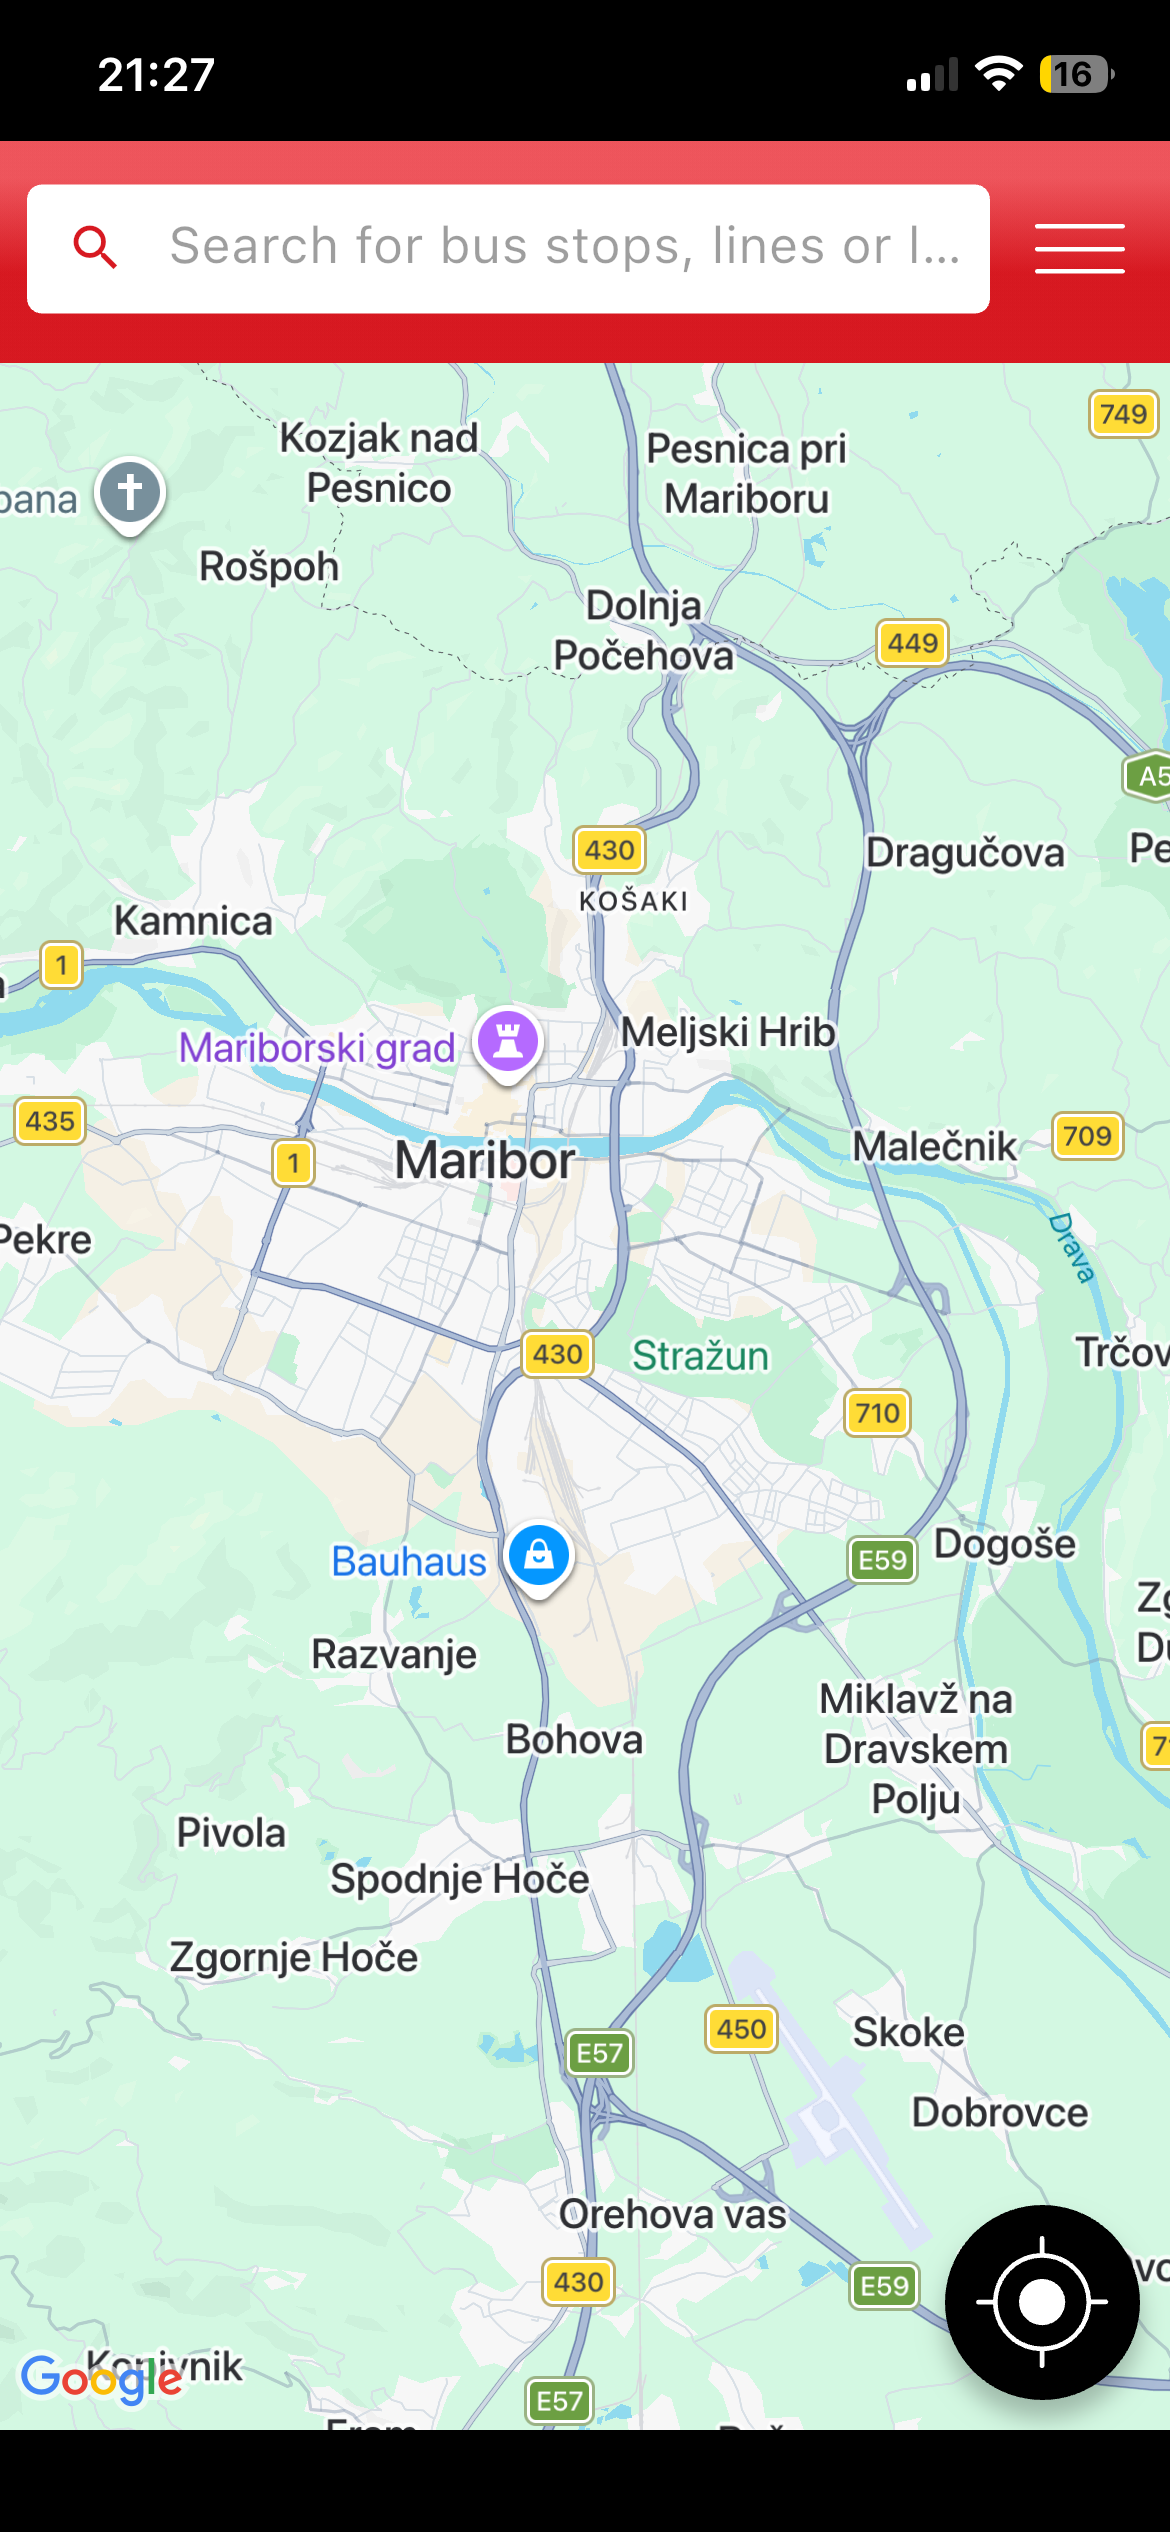
\includegraphics[width=0.8\textwidth]{mobilnost.png}
\caption{Mobilna aplikacija M mobilnost}
\end{figure}

\section{Marprom Shop}

Marprom Shop omogoča spletni in mobilni
nakup avtobusnih vozovnic \cite{shop}.

\textbf{Funkcionalnosti:}
Nakup vozovnic, polnjenje kartic
in uporaba vozovnic na telefonu.

\textbf{Prednosti:}
Nakup vozovnic brez obiska blagajne.

\textbf{Slabosti:}
Za nakup potrebujemo ustrezno
elektronsko plačilno sredstvo.

\begin{figure}[h]
\centering
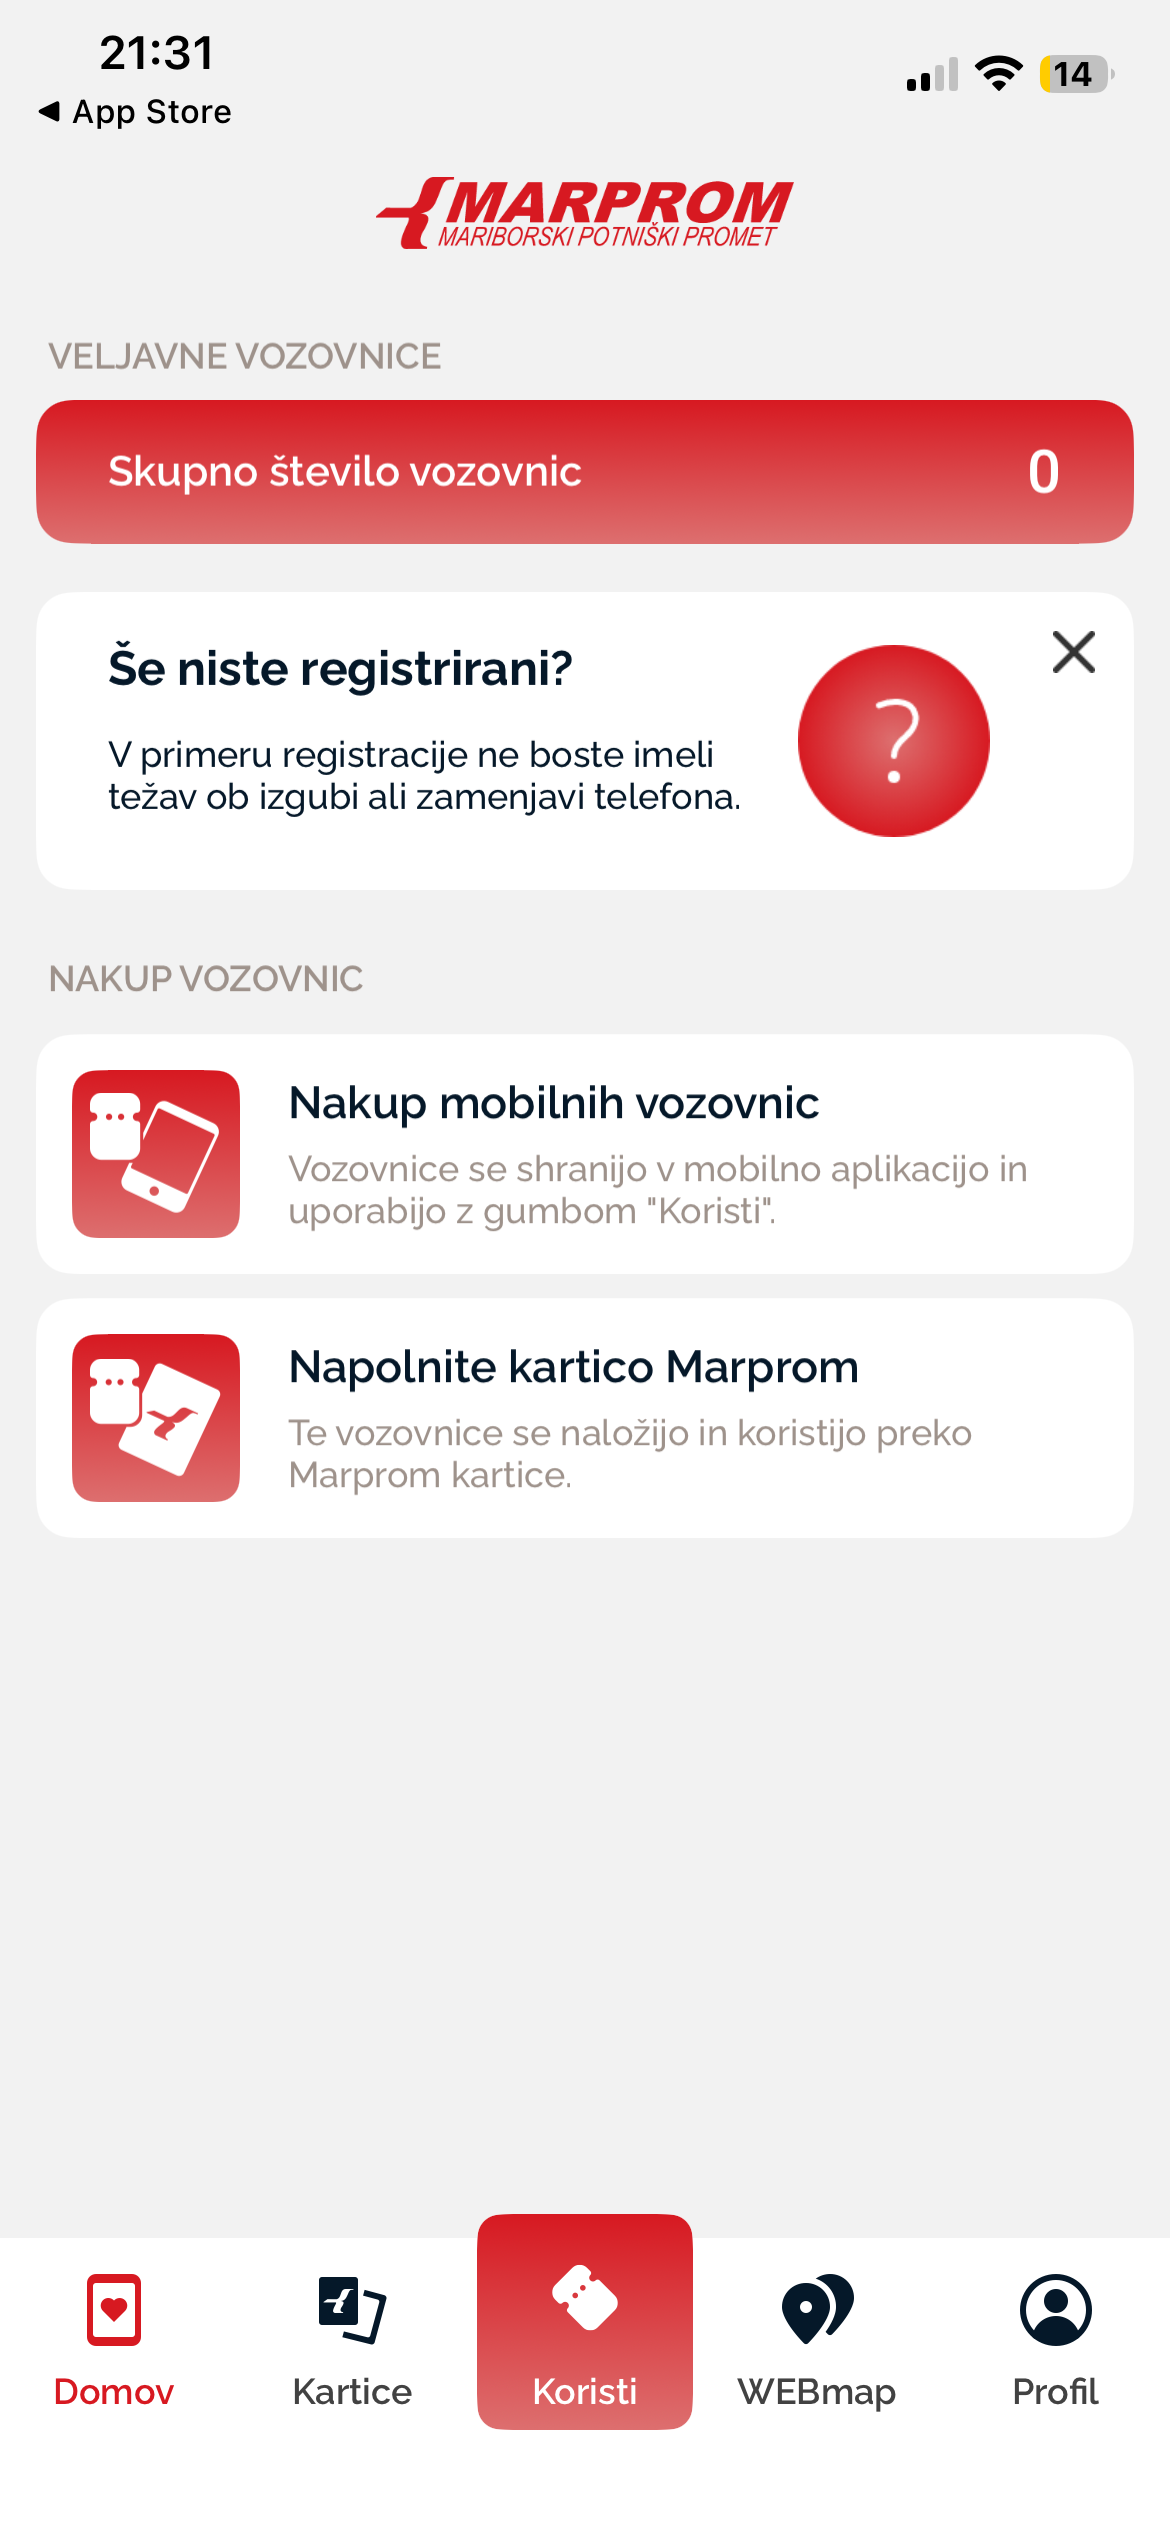
\includegraphics[width=0.8\textwidth]{shop.png}
\caption{Marprom Shop}
\end{figure}

\section{Zaključek}

Pregledali smo tri digitalne storitve
podjetja Marprom.

Interaktivni vozni redi omogočajo pregled
odhodov, M mobilnost spremljanje avtobusov,
Marprom Shop pa nakup vozovnic.

Pri našem projektu želimo te funkcionalnosti
povezati v pregleden uporabniški vmesnik,
kjer bi uporabnik na enem mestu našel
najpomembnejše informacije.

\begin{thebibliography}{9}

\bibitem{vozniredi}
Marprom, Interaktivni vozni redi.
\url{https://vozniredi.marprom.si/}

\bibitem{mobilnost}
Marprom, M mobilnost.
\url{https://www.marprom.si/e-storitve/m-mobilnost/}

\bibitem{shop}
Marprom, Marprom Shop.
\url{https://www.marprom.si/e-storitve/marprom-shop/}

\end{thebibliography}

\end{document}


\title{Marprom - Pregled obstoječih rešitev}
\author{Leon Bracko, Tijan Eisenhut List}
\date{November 2026}
\maketitle

\section{Uvod}

Naš projekt je povezan z mestnim avtobusnim
prometom Marprom v Mariboru.

Namen projekta je uporabnikom omogočiti
enostaven pregled voznih redov, avtobusnih
linij in drugih informacij o prevozu.

Pregledali smo tri obstoječe digitalne
storitve podjetja Marprom.

\section{Interaktivni vozni redi}

Interaktivni vozni redi omogočajo pregled
avtobusnih linij in odhodov v Mariboru
\cite{vozniredi}.

\textbf{Funkcionalnosti:}
Pregled linij, postajališč in voznih redov.

\textbf{Prednosti:}
Enostaven dostop do informacij o odhodih.

\textbf{Slabosti:}
Za uporabo je potrebna internetna povezava.

\begin{figure}[h]
\centering
\includegraphics[width=0.8\textwidth]{slike/vozniredi.png}
\caption{Interaktivni vozni redi Marprom}
\end{figure}

\section{M mobilnost}

M mobilnost je mobilna aplikacija za
spremljanje avtobusnega prometa v
Mariboru \cite{mobilnost}.

\textbf{Funkcionalnosti:}
Prikaz avtobusov v realnem času,
pregled odhodov in načrtovanje poti.

\textbf{Prednosti:}
Uporabnik lahko spremlja položaj
avtobusa na zemljevidu.

\textbf{Slabosti:}
Za uporabo potrebujemo pametni telefon
in internetno povezavo.

\begin{figure}[h]
\centering
\includegraphics[width=0.8\textwidth]{slike/mobilnost.png}
\caption{Mobilna aplikacija M mobilnost}
\end{figure}

\section{Marprom Shop}

Marprom Shop omogoča spletni in mobilni
nakup avtobusnih vozovnic \cite{shop}.

\textbf{Funkcionalnosti:}
Nakup vozovnic, polnjenje kartic
in uporaba vozovnic na telefonu.

\textbf{Prednosti:}
Nakup vozovnic brez obiska blagajne.

\textbf{Slabosti:}
Za nakup potrebujemo ustrezno
elektronsko plačilno sredstvo.

\begin{figure}[h]
\centering
\includegraphics[width=0.8\textwidth]{slike/shop.png}
\caption{Marprom Shop}
\end{figure}

\section{Zaključek}

Pregledali smo tri digitalne storitve
podjetja Marprom.

Interaktivni vozni redi omogočajo pregled
odhodov, M mobilnost spremljanje avtobusov,
Marprom Shop pa nakup vozovnic.

Pri našem projektu želimo te funkcionalnosti
povezati v pregleden uporabniški vmesnik,
kjer bi uporabnik na enem mestu našel
najpomembnejše informacije.

\begin{thebibliography}{9}

\bibitem{vozniredi}
Marprom, Interaktivni vozni redi.
\url{https://vozniredi.marprom.si/}

\bibitem{mobilnost}
Marprom, M mobilnost.
\url{https://www.marprom.si/e-storitve/m-mobilnost/}

\bibitem{shop}
Marprom, Marprom Shop.
\url{https://www.marprom.si/e-storitve/marprom-shop/}

\end{thebibliography}

\end{document}
